\chapter*{Samenvatting}
\addcontentsline{toc}{chapter}{Samenvatting}

{\selectlanguage{dutch}

\noindent 
\dropcap{D}{eze} Nederlandse samenvatting is speciaal geschreven
voor niet-biologen, zodat zij een beter idee kunnen
krijgen wat er in dit proefschrift besproken wordt.

\paragraph{Soortvorming}

Er zijn op de wereld veel verschillende (dier-, plant-, etc.) soorten.
Helemaal in het begin van het ontstaan van de Aarde, 
was dit nog niet zo, want toen ontstonden de eerste soorten.
In de loop van de tijd zijn er heel veel soorten bijgekomen.
Het proces die dat doet, noemen we soortvorming.

\paragraph{Soortvorming in bacteriën}

Soortvorming kan op meerdere manieren gebeuren.
In bacterieën zeggen we dat twee bacteriën verschillend zijn,
als hun DNA genoeg verschilt. Bacteriën vermenigvuldigen zichzelf
als de omstandigheden gunstig zijn en bij elke celding vinden
er veranderingen in het DNA plaats. Als je twee identieke bacteriën
lang genoeg laat delen, heb je na een tijd twee verschillende 
bacteriesoorten.

\paragraph{Soortvorming in vooral dieren}

Bij dieren is het moeilijker te zeggen wanneer twee dieren
verschillende soorten zijn. Een veelgebruikte definitie is dat
twee groepen dieren verschillende diersoorten zijn, als een kruising
tussen de twee groepen geen of onvruchtbare kleinkinderen oplevert.

Er zijn meerdere mechanismen die ervoor zorgen 
dat soortvorming in dieren plaatsvind. 
Een simpel mechanisme is dat een groep dieren een tweeën gesplits
wordt door een verandering in het landschap, 
zoals een rivier of bergketen.

\paragraph{Fylogenieën}

Als we kijken naar een verzameling soorten over langere tijd (denk
aan miljoenen jaren!), dan zal er waarschijnlijk 
soortvorming plaatsvinden. Sommige soorten zullen meer nieuwe soorten
dan anderen opleveren. We kunnen dit proces laten zien met een
fylogenetische boom, zoals bijvoorbeeld in figuur \ref{fig:fylogenie}.

\begin{figure}
  \centering
  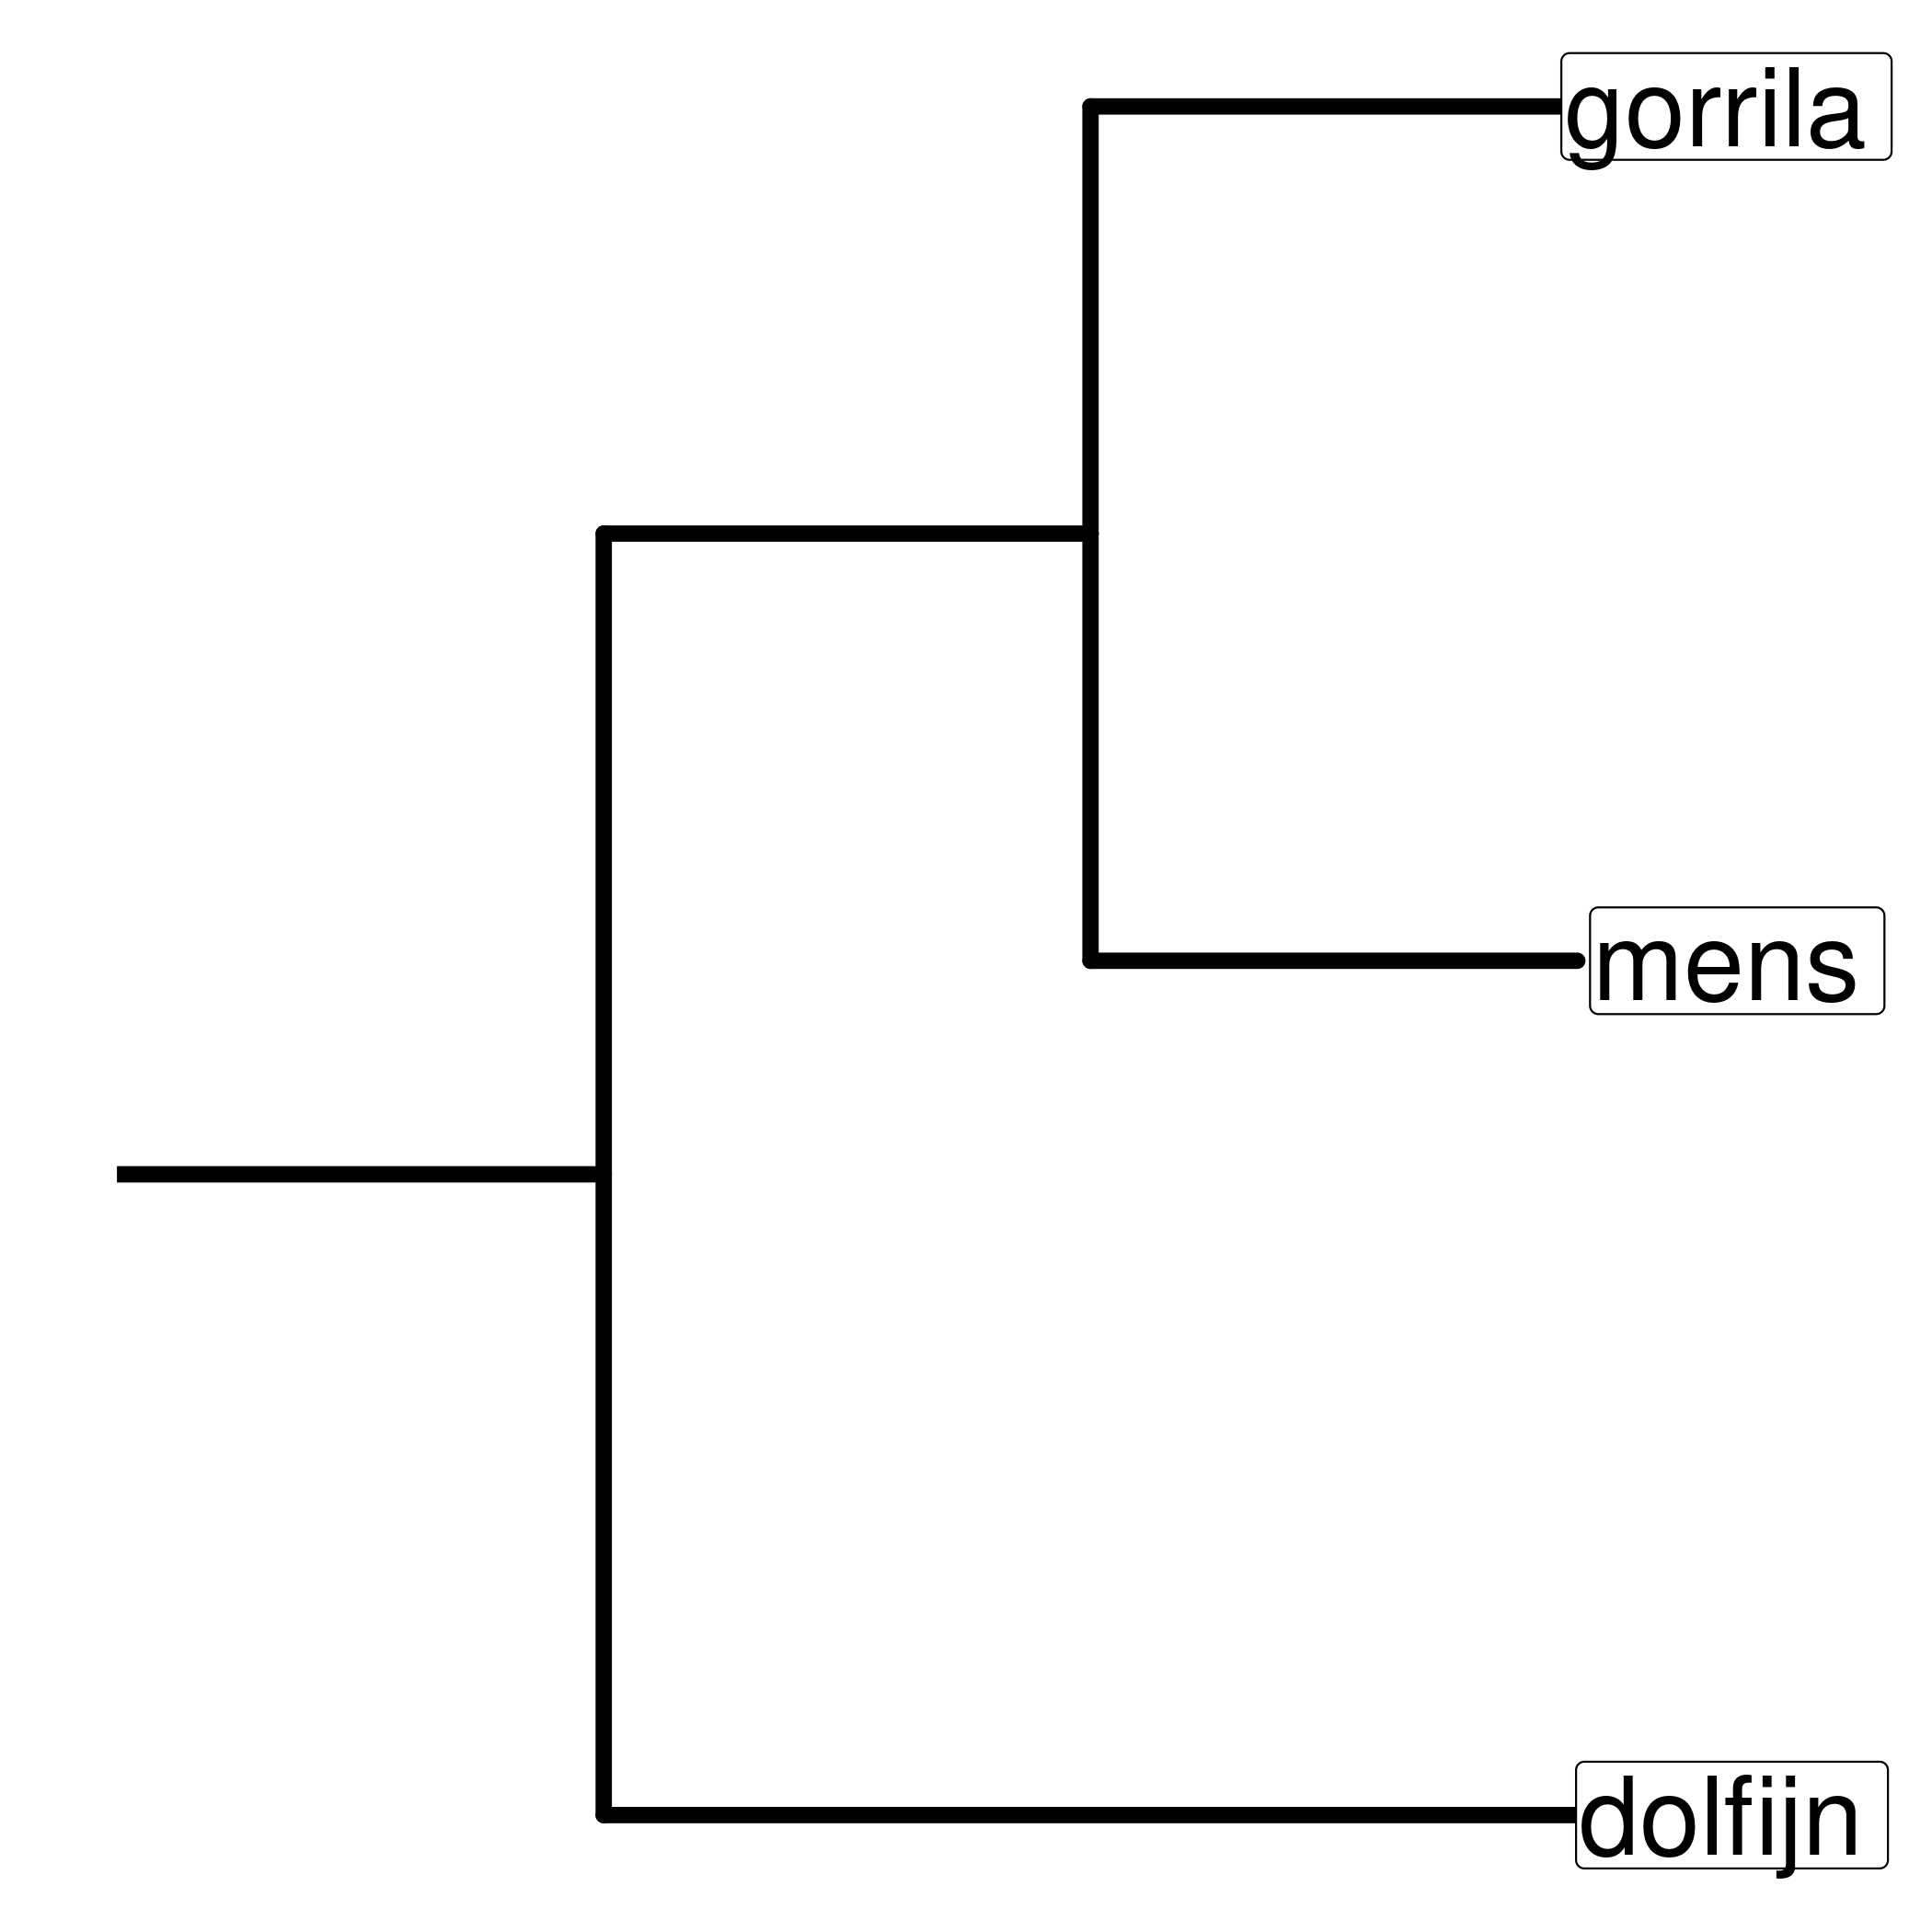
\includegraphics[width=0.5\textwidth]{fylogenie.png}
  \caption{
    Een fylogenie die laat zien dat mensen en gorilla's 
    meer aan elkaar verwant zijn dan mensen en dolfijnen.
    Deze fylogenie is niet op schaal.
  }
  \label{fig:fylogenie}
\end{figure}

\paragraph{DNA}

Er is informatie nodig om een fylogenie te kunnen maken,
bijvoorbeeld de DNA volgorde van de soorten in de fylogenie.
Alle levende wezens hebben DNA, waardoor het mogelijk is alle
soorten in een grote fylogenie te zetten.
Elke keer dat DNA wordt doorgegeven aan de volgende generatie,
verandert de DNA volgorde een klein beetje. 
Deze eigenschap maakt het mogelijk om een fylogenie te
kunnen baseren op DNA volgordes.
Simpel gezegt: de soorten waarvan de DNA volgordes het meest op elkaar
lijken, zijn meer aan elkaar verwant.

\paragraph{Fylogenetisch model}

Er zijn meerdere manieren om een fylogenie te berekenen 
aan de hand van DNA volgordes, omdat je verschillende
aannames kunt hebben over hoe soortvorming plaatsvind.
Je kunt bijvoorbeeld aannemen dat soortvorming gemiddeld altijd
even vaak optreedt. Of dat DNA in alle soorten altijd even snel
verandert. De verzameling van aannames noemen we een model,
in dit geval noemen we dit een fylogenetisch model.

\paragraph{Fylogenieën maken}

Er zijn computerprogramma's die van een fylogenetisch model en DNA
sequensies een fylogenie kunnen maken. Eén van de populairste is
het programma BEAST2. Omdat ik veel fylogenieën zou gaan maken, 
was het voor mij belangrijk dat ik dit met enkel code (dus zonder 
muisklikken) zou kunnen doen. Daarom heb ik \verb;babette;
geprogrammeert, een R package waarmee je BEAST2 kunt aanroepen.
In hoofdstuk 2 kun je lezen over \verb;babette;.

\paragraph{Fylogenetische modellen}

Omdat je veel aannames kunt maken over hoe soortvorming plaatsvindt,
is het de vraag welke de beste verzameling aannames is.
En ook het vergelijken van fylogenetische modellen (om uit te vinden
welke 'de beste' is) kan op meerdere manieren. 
Een nadeel van de meeste manieren is dat het fylogenetische model
wiskundig goed onderzocht moet zijn. 
Dit betekent dat je eerst een nieuw fylogenetisch model moet oplossen,
voor je kunt weten hoe goed dat model is.

\paragraph{Kijken hoe goed fylogenetische modellen zijn}

Met een groepje van drie hebben wij een manier bedacht om
te kijken of het wel belangrijk is om een nieuw fylogenetisch
model wiskundig op te lossen.
Met onze manier hoef je alleen maar een boel fylogenieën
van het nieuw model te simuleren.
Dit is vaak veel gemakkelijker dan een model wiskundig op te lossen.
Deze manier hebben we in een R package gestopt, die we
\verb;pirouette; hebben genoemd. In hoofdstuk 3 kun je lezen
over \verb;pirouette;.

\paragraph{Een nieuw soortvormingsmodel testen}

Toen we een manier hadden om te kijken hoe belangrijk het is om
een fylogenetisch model wiskundig op te lossen, gingen
we dit gebruiken op een nieuw fylogenetisch model,
dat nog niet wiskundig is opgelost.

Dit nieuwe model heet het MBD ('Multiple-Birth Death') model.
Binnen dit model is de aanname dat soortvorming altijd voor
alle soorten even vaak voorkomt, maar dat er soms een 
'geboortegolf' optreedt, waarin er in meerdere soorten tegelijk 
soortvorming optreedt. 

In hoofdstukken 4 kun je lezen hoe we dit precies hebben gedaan.
We kwamen erachter dat dit nieuwe en ingewikkeldere model
niet veel beter is dan de simpelere modellen die wiskundig al
zijn opgelost. Als je alleen maar goeie fylogenieën wilt krijgen,
is het dus niet nodig het MBD model op te lossen.

\paragraph{Conclusie}

Dit proefschrift leert ons dat we kunnen weten of we een nieuw fylogenetisch
model zouden moeten onderzoeken, waardoor wetenschappers 
nuttigere dingen kunnen doen.

Het mooie aan mijn onderzoek is dat andere wetenschappers er zelf gemakkelijk 
ook wat mee kunnen:
met \verb;babette; kan iedereen gemakkelijk fylogenieen maken uit DNA
sequenties. Op het moment van schrijven zijn er 3 wetenschappelijk artikelen
gepubliceerd die \verb;babette; gebruiken.
Ook \verb;pirouette; is een sterk R package geworden, maar er zijn
nog geen publicaties die het gebruiken.

} % ~\selectlanguage{dutch}
